\documentclass[11pt]{article}

\usepackage{amssymb}
\usepackage{amsmath}
\usepackage{multicol}
\usepackage{graphicx}
\usepackage{epigraph}
\usepackage{chngpage}
\usepackage{fancyhdr}
\usepackage[braket, qm]{qcircuit}
\usepackage[font=small,labelfont=bf]{caption}
\usepackage[hidelinks]{hyperref}
\usepackage{subcaption}
\usepackage[normalem]{ulem}
\usepackage{tikz}

\usepgflibrary{arrows}

%% Gate matrices and quantum state vectors
\newcommand{\igate}{
  \begin{bmatrix}
  1 & 0 \\
  0 & 1
  \end{bmatrix}
}
\newcommand{\xgate}{
  \begin{bmatrix}
  0 & 1 \\
  1 & 0
  \end{bmatrix}
}
\newcommand{\ygate}{
  \begin{bmatrix}
  0 & -i \\
  i & \phantom{-}0
  \end{bmatrix}
}
\newcommand{\zgate}{
  \begin{bmatrix}
  1 & \phantom{-}0 \\
  0 & -1
  \end{bmatrix}
}
\newcommand{\hgate}{
  \dfrac{1}{\sqrt2}
  \begin{bmatrix}
  1 & \phantom{-}1 \\
  1 & -1
  \end{bmatrix}
}
\newcommand{\sgate}{
  \begin{bmatrix}
  1 & 0 \\
  0 & i
  \end{bmatrix}
}
\newcommand{\cnotgate}{
  \begin{bmatrix}
  1 & 0 & 0 & 0 \\
  0 & 1 & 0 & 0 \\
  0 & 0 & 0 & 1 \\
  0 & 0 & 1 & 0 \\
  \end{bmatrix}
}

\newcommand{\qstatezero}{
  \begin{bmatrix}1 \\ 0\end{bmatrix}
}
\newcommand{\qstateone}{
  \begin{bmatrix}0 \\ 1\end{bmatrix}
}

\setlength\epigraphwidth{10cm}
\setlength\epigraphrule{0pt}

\usepackage{etoolbox}

\makeatletter
\patchcmd{\epigraph}{\@epitext{#1}}{\itshape\@epitext{#1}}{}{}
\makeatother

\renewcommand*{\arraystretch}{1.15}

\pagestyle{fancy}
\lhead{}

\title{\textbf{Introduction to Quantum Computing \\
\large Lectures by Leon Riesebos}}
\author{Steven Oud \\ \emph{soud@pm.me}}
\begin{document}

\vfill
\maketitle

\tableofcontents

\newpage

\section{Fundementals: A One-Qubit World}
\epigraph{Quantum computers are machines that rely on characteristically quantum phenomena, such as quantum interference and quantum entanglement, in order to perform computation.}{--- Artur Ekert}

\epigraph{It is tempting to say that a quantum computer is one whose operation is governed by the laws of quantum mechanics. But since the laws of quantum mechanics govern the behavior of all physical phenomena, this temptation must be resisted. Your laptop operates under the laws of quantum mechanics, but it is not a quantum computer.}{--- N. David Mermin}

\subsection{The Qubit}
A qubit - like a classical bit - has a \emph{state}. In classical bits, this is 0 or 1. Two possible states for a qubit are \ket{0} and \ket{1} (called \emph{Dirac notation}), which correspond to the states 0 and 1 for a classical bit. The difference between bits and qubits is that a qubit can be in other states than \ket{0} or \ket{1}, often called \emph{superpositions}. The state of a qubit can be denoted as following:
\[\ket{\psi} = \alpha\ket{0} + \beta\ket{1}\]
where $\alpha$ and $\beta$ are complex numbers. The special states \ket{0} and \ket{1} are known as \emph{computational basis states}. We cannot examine a qubit to determine its quantum state. Quantum mechanics tells us we can only acquire much more restricted information about the quantum state. When we measure a qubit we get either 0, with probability $|\alpha|^2$, or 1, with probability $|\beta|^2$. The sum of all probabilities is always equal to 1:
\[|\alpha|^2 + |\beta|^2 = 1\]
For example, a qubit in the state
\[
\dfrac{1}{\sqrt2}\ket{0}+\dfrac{1}{\sqrt2}\ket{1}
\]
gives 0 fifty percent of the time ($|1/\sqrt2|^2$), and 1 fifty percent of the time. This state is often denoted by \ket{+}.
\newpage
\subsection{Bloch Sphere}
The Bloch sphere is a geometrical representation of a qubit's state. It's a spherical coordinate system in which a quantum state can be described as following:
\[
  \ket{\psi} = e^{i\delta} \left(cos\dfrac{\theta}{2}\ket{0} + e^{i\phi}sin\dfrac{\theta}{2}\ket{1}\right)
\]
where $\delta, \theta$ and $\phi$ are real numbers. We can ignore the factor $e^{i\delta}$ out the front, because it has no observable effect, allowing us to write
\[
  \ket{\psi} = cos\dfrac{\theta}{2}\ket{0} + e^{i\phi}sin\dfrac{\theta}{2}\ket{1}
\]
The numbers $\theta$ and $\phi$ define a point on the three-dimensional sphere (Figure~\ref{fig:bloch}). The Bloch sphere visualization can be very useful for describing single qubit operations. It is however limited in that there is no simple generalization of the Bloch sphere known for multiple qubits.
\begin{figure}[ht]
  \centering
  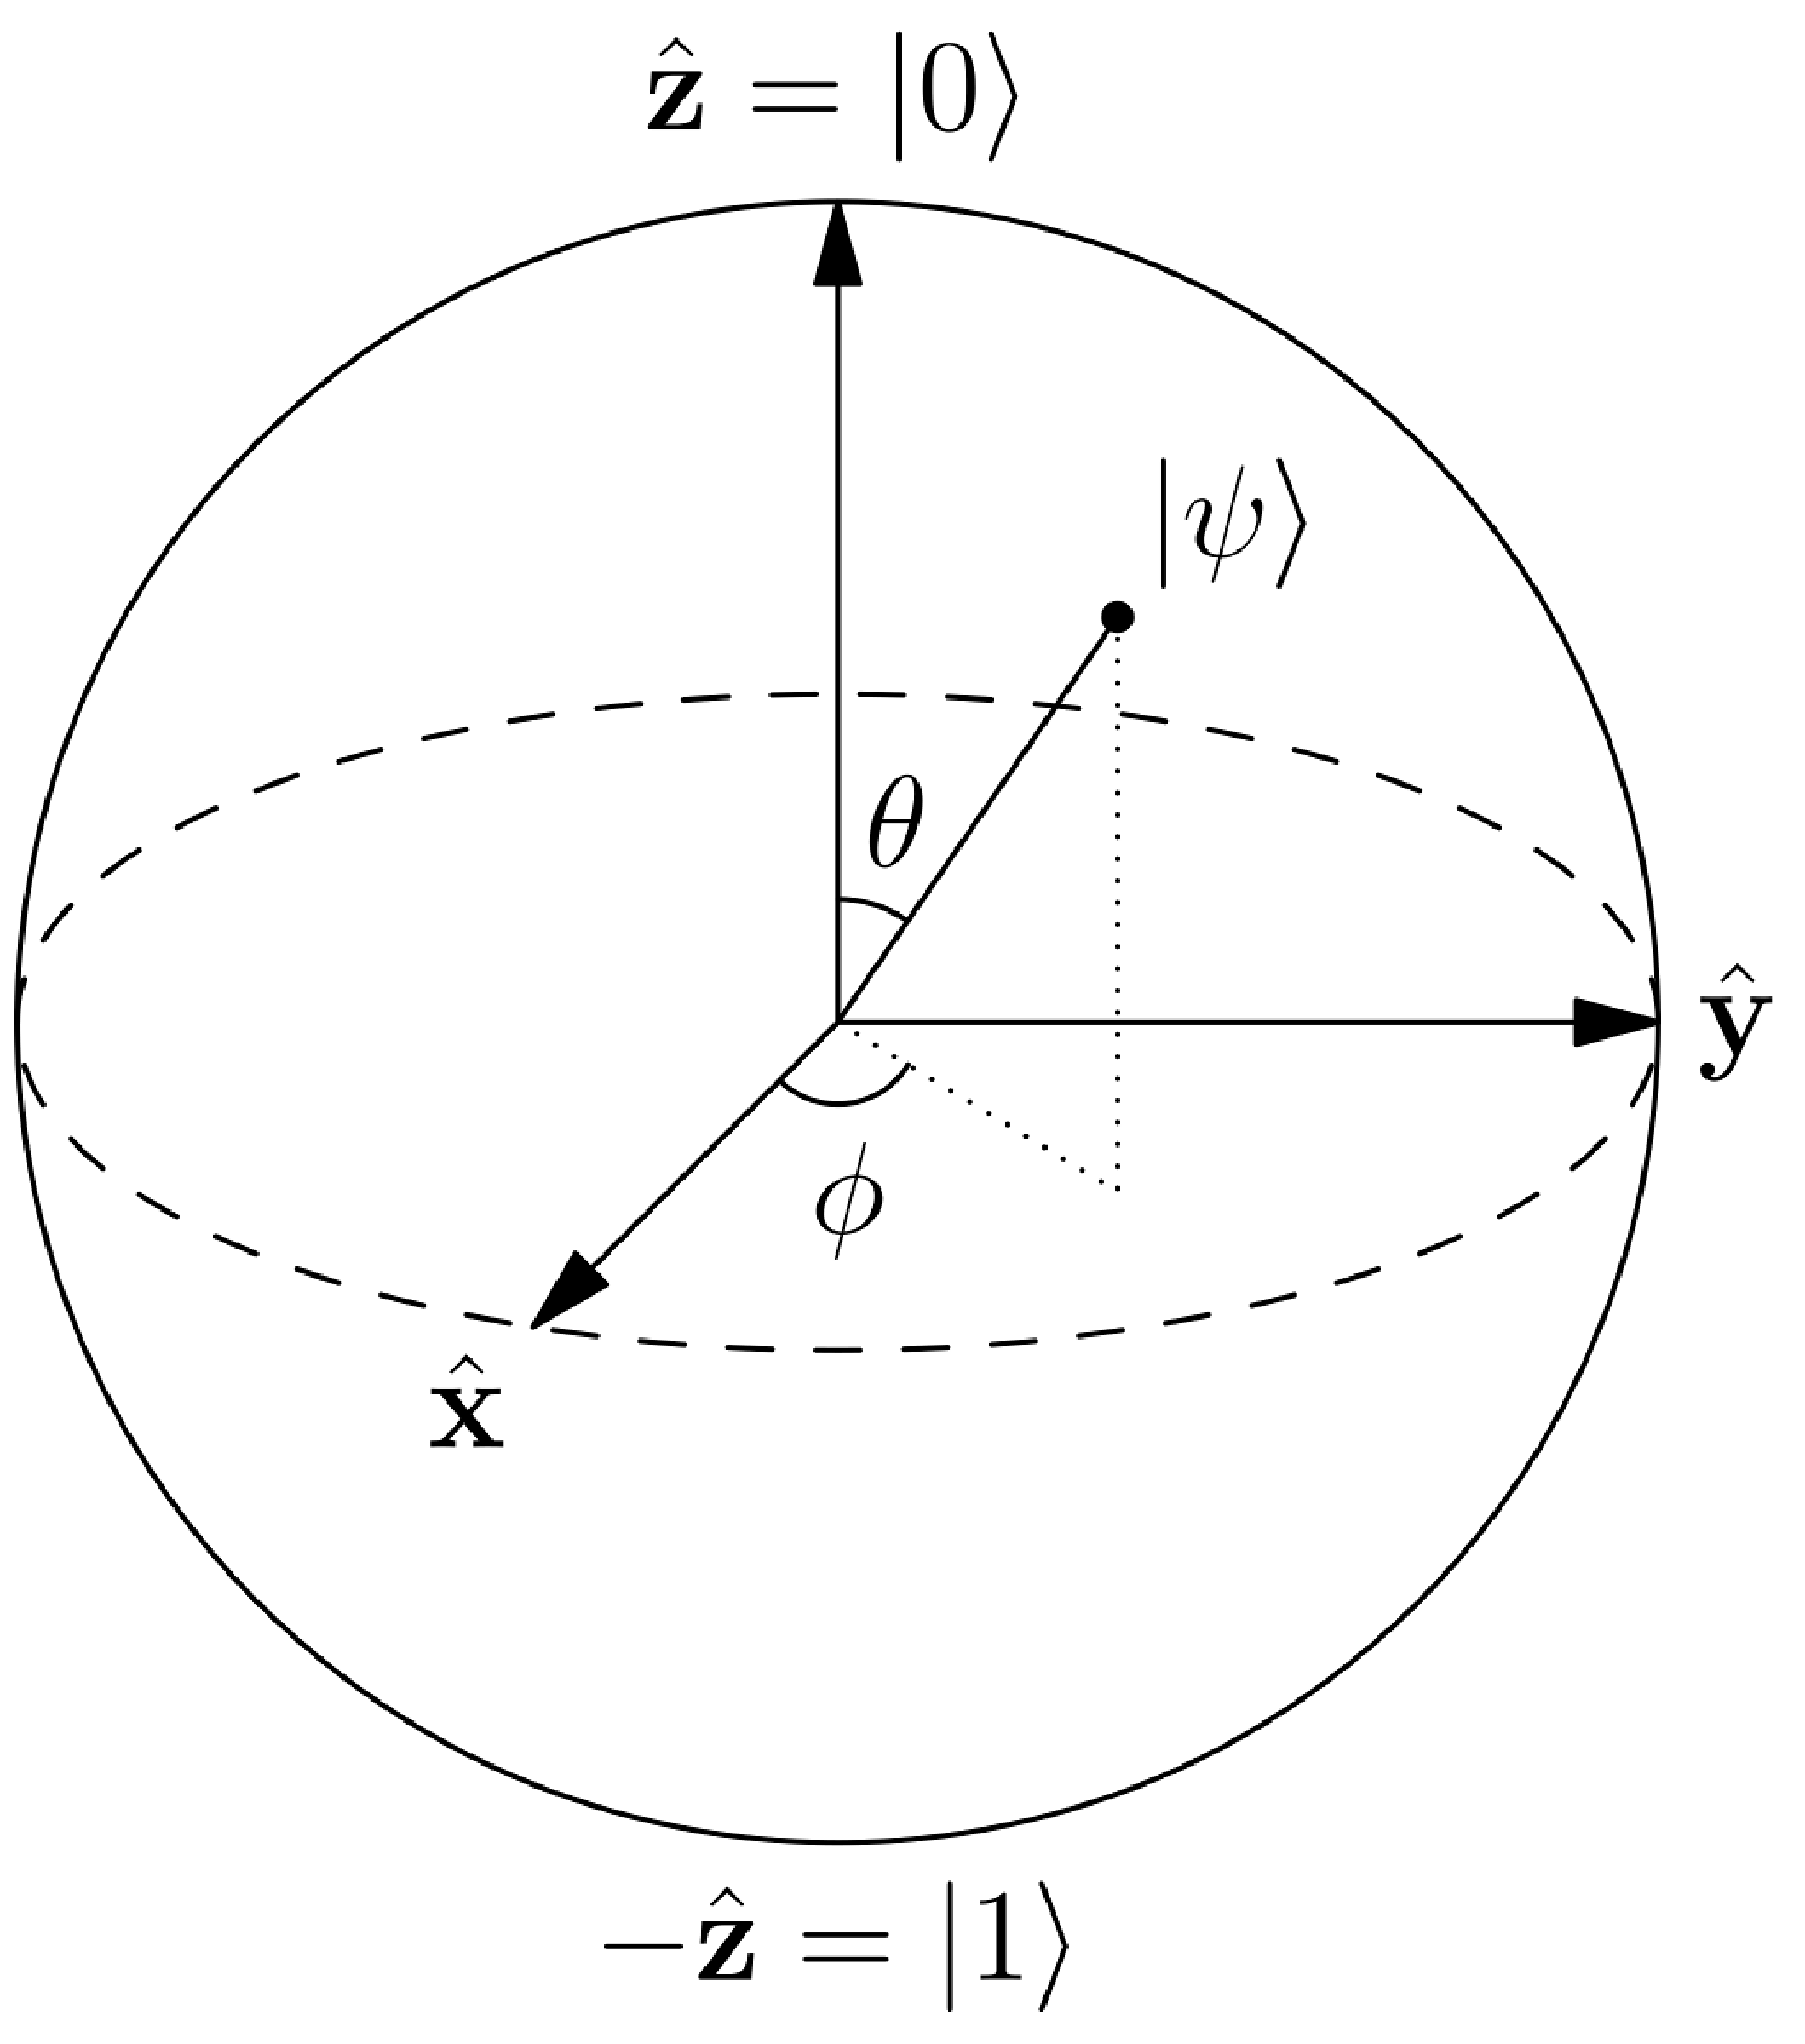
\includegraphics[scale=0.2]{images/bloch_sphere.eps}
  \caption{Bloch sphere representation of a qubit.}
  \label{fig:bloch}
\end{figure}
\par
\newpage

\subsection{Single-Qubit Quantum Operations}
Single-qubit quantum gates can be seen as rotations on the Bloch sphere. Quantum gates can be represented by matrices, which we will look at in Section~\ref{sec:matrix_notation}. These gates only have one limitation: they have to be \emph{unitary}, that is $U^\dagger U = I$, where $U^\dagger$ is the Hermitian adjoint of $U$. Therefore, any $2^n \times 2^n$ unitary matrix is a valid gate which acts on $n$ qubits. Below are some notable single-qubit gates described and visualized.

\subsubsection{Pauli Gates}
 The most simple quantum gates are the \emph{Pauli} gates $I$, $X$, $Y$ and $Z$. $I$ is the identity gate, which does nothing. The other gates rotate $\pi$ radians (180 degrees) around the X, Y or Z-axis. These gates are self-inverse, meaning $U^2 = I$.

\begin{figure}[ht]
  \begin{adjustwidth}{-2.5cm}{-2.5cm}
  \centering
  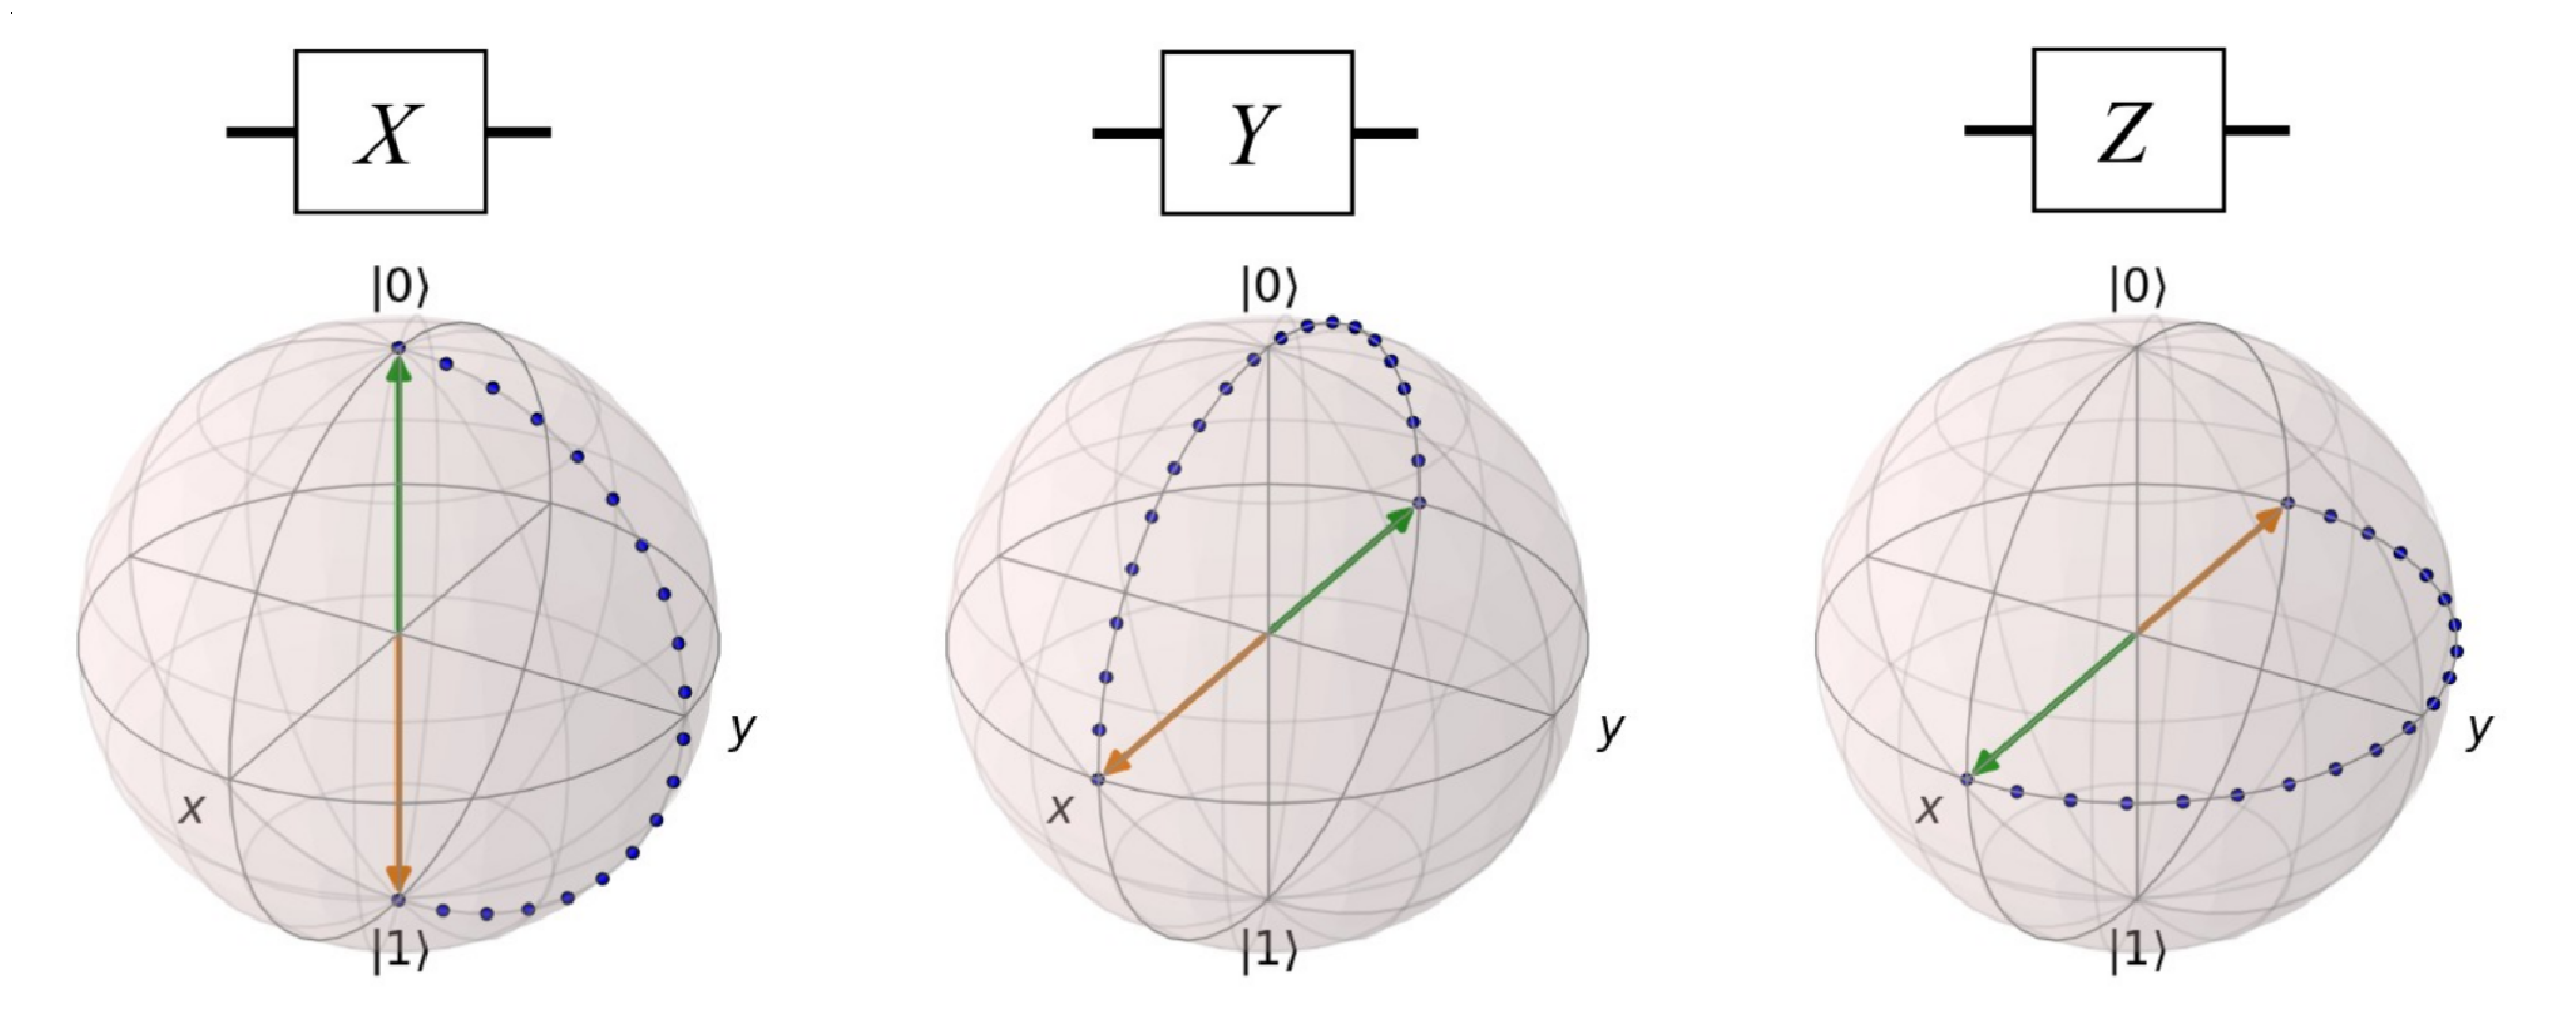
\includegraphics[scale=0.25]{images/pauli_gates.eps}
  \caption{Pauli gates $X$, $Y$ and $Z$ visualized on the Bloch sphere.}
  \end{adjustwidth}
\end{figure}


\subsubsection{S Gate}
The \emph{S} gate, also known as the phase ($P$) gate, does a Z rotation of $\pi/2$ radians (90 degrees). It's essentially half a Pauli Z gate. The S gate belongs to the Clifford gates.

\begin{center}
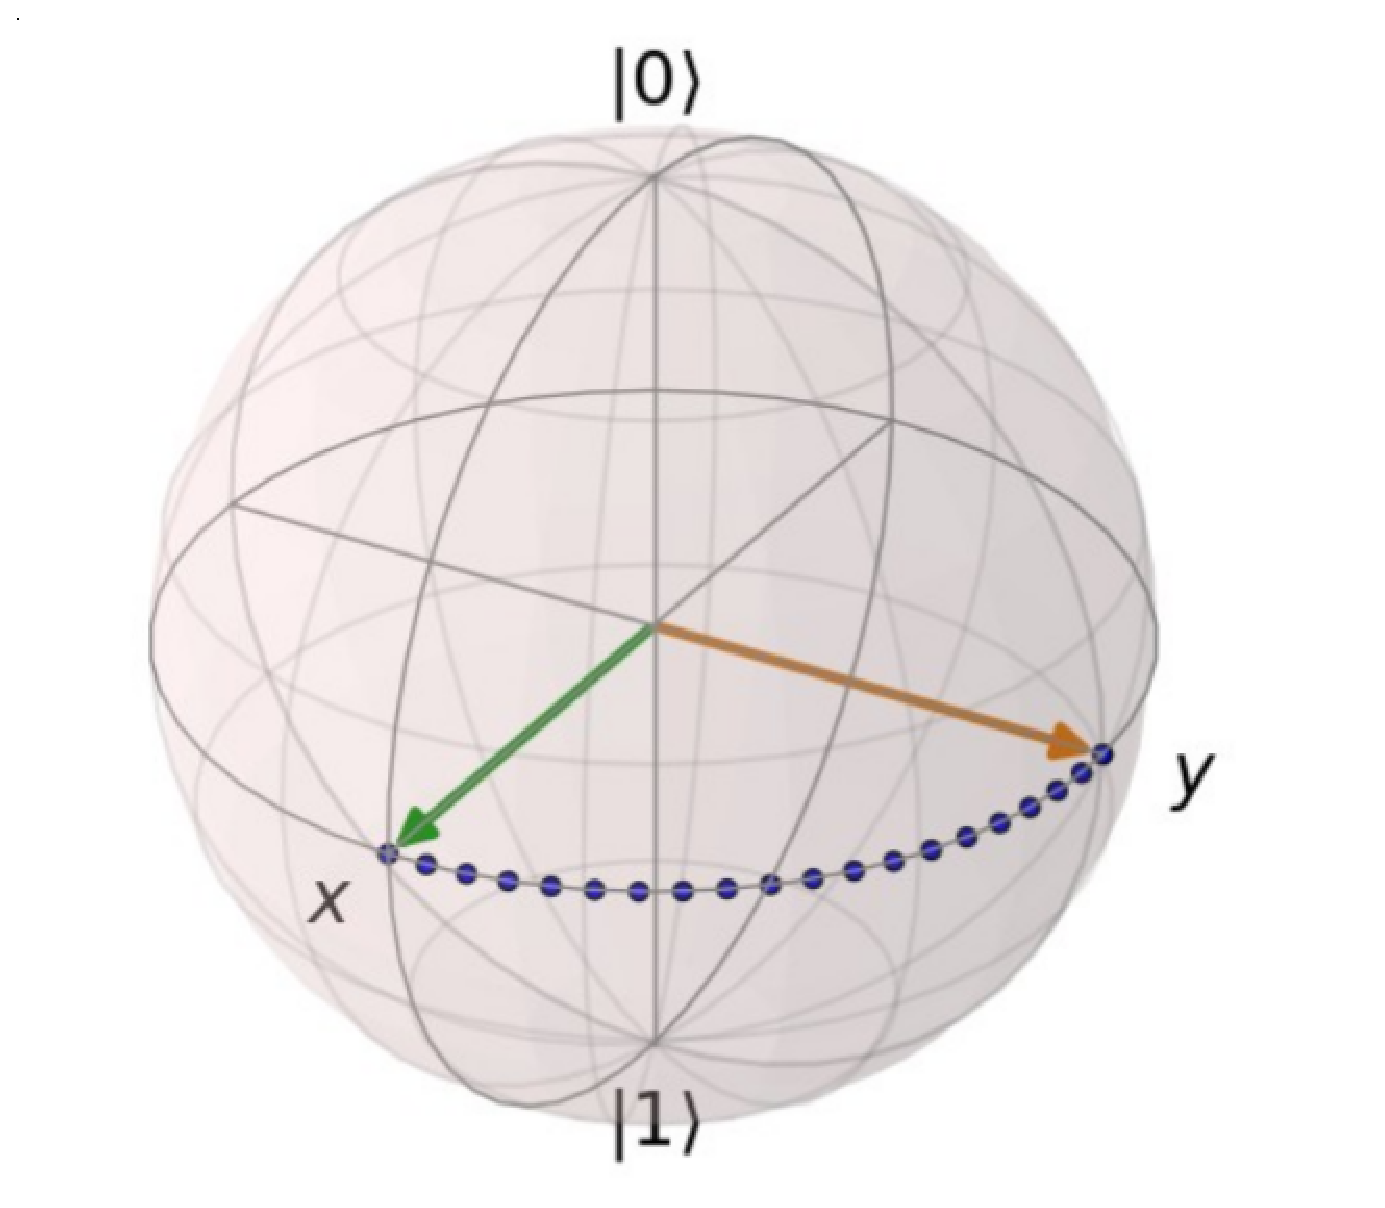
\includegraphics[scale=0.30]{images/s_gate.eps}
\end{center}

\subsubsection{Hadamard Gate}
The Hadamard ($H$) gate maps the qubit-basis states $\ket{0}$ and $\ket{1}$ to superposition states with equal weight. It is the combination of two rotations, $\pi$ radians about the Z-axis followed by $\pi/2$ radians about the Y-axis.

This gate is sometimes described as a ``square root of $NOT$" gate, because it turns $\ket{0}$ into $(\ket{0} + \ket{1})/\sqrt2$ (also written as $\ket{+}$), halfway between $\ket{0}$ and $\ket{1}$. The Hadamard gate also belongs to the Clifford gates.

\begin{figure}[ht]
  \centering
  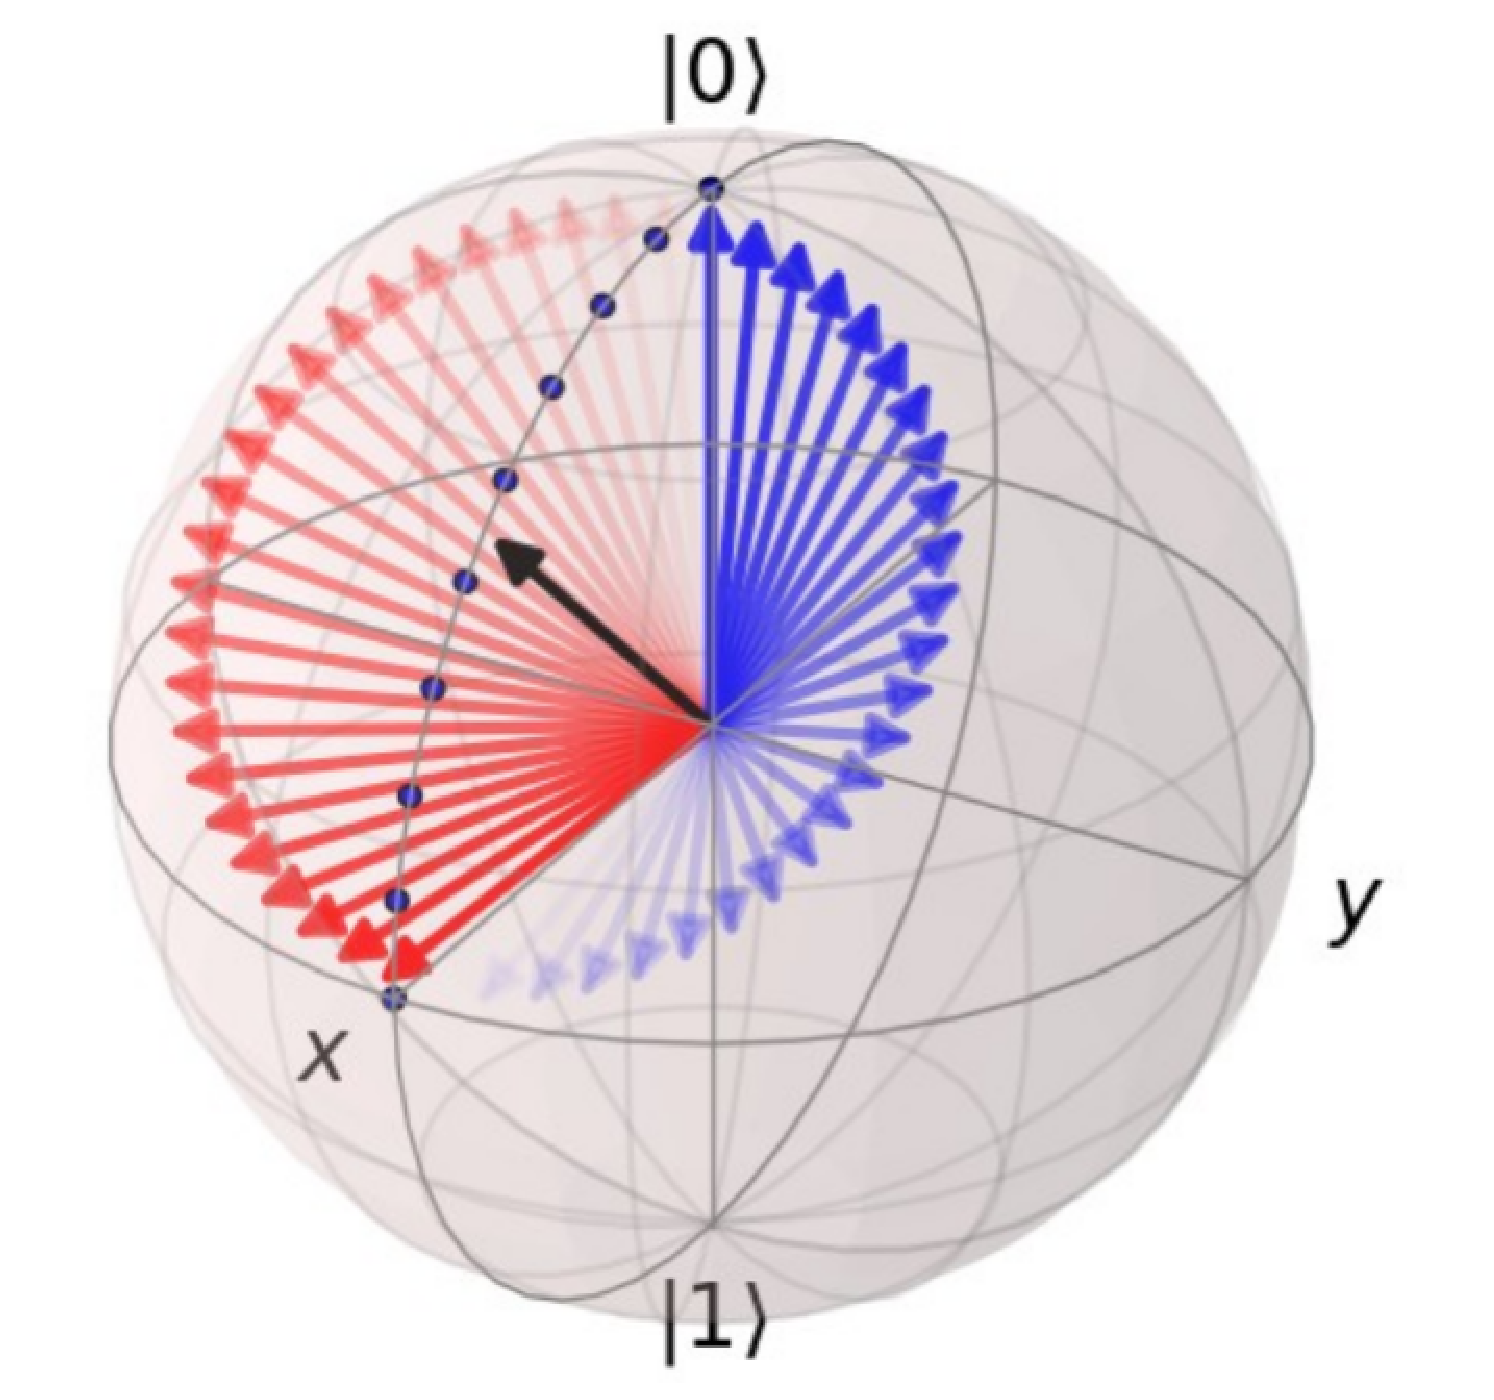
\includegraphics[scale=0.25]{images/hadamard_gate.eps}
  \caption{Hadamard gate visualized on the Bloch sphere.}
\end{figure}

\subsection{Measurement}
Measuring a qubit collapses its state. The probabilistic result of a qubit measurement can be calculated based on the probability amplitudes:
\[\ket{\psi} = \alpha\ket{0} + \beta\ket{1}\]
\[P(\ket{0}) = \left|\alpha\right|^2\]
\[P(\ket{1}) = \left|\beta\right|^2\]
Consider the following simple single-qubit circuit:

\begin{figure}[ht]
\[
  \Large{
    \Qcircuit @C=1em @R=0em {
    \push{\rule{0em}{1em}} & & \lstick{\ket{0}} & \gate{H} & \gate{Z} & \meter & \cw
    }
  }
\]
\caption{A simple quantum circuit. The output of measuring a qubit is a classical bit, which is distinguished from a qubit by drawing a double-line wire. A visualization of this circuit on the Bloch sphere can be seen in Figure~\ref{fig:gate_rotations}.}
\end{figure}
\noindent
We start with computing $H\ket{0} = \ket{+}$, followed by $Z\ket{+} = \ket{-}$. Finally we measure. We can calculate the probabilities:
\[\ket{-} = \dfrac{1}{\sqrt2} (\ket{0} - \ket{1})\]
\[P(\ket{0}) = \left|\dfrac{1}{\sqrt2}\right|^2 = \dfrac{1}{2}\]
\[P(\ket{1}) = \left|\dfrac{-1}{\sqrt2}\right|^2 = \dfrac{1}{2}\]
Giving us equal probabilities of our state being measured as $\ket{0}$ or $\ket{1}$.

\begin{figure}[ht]
  \centering
  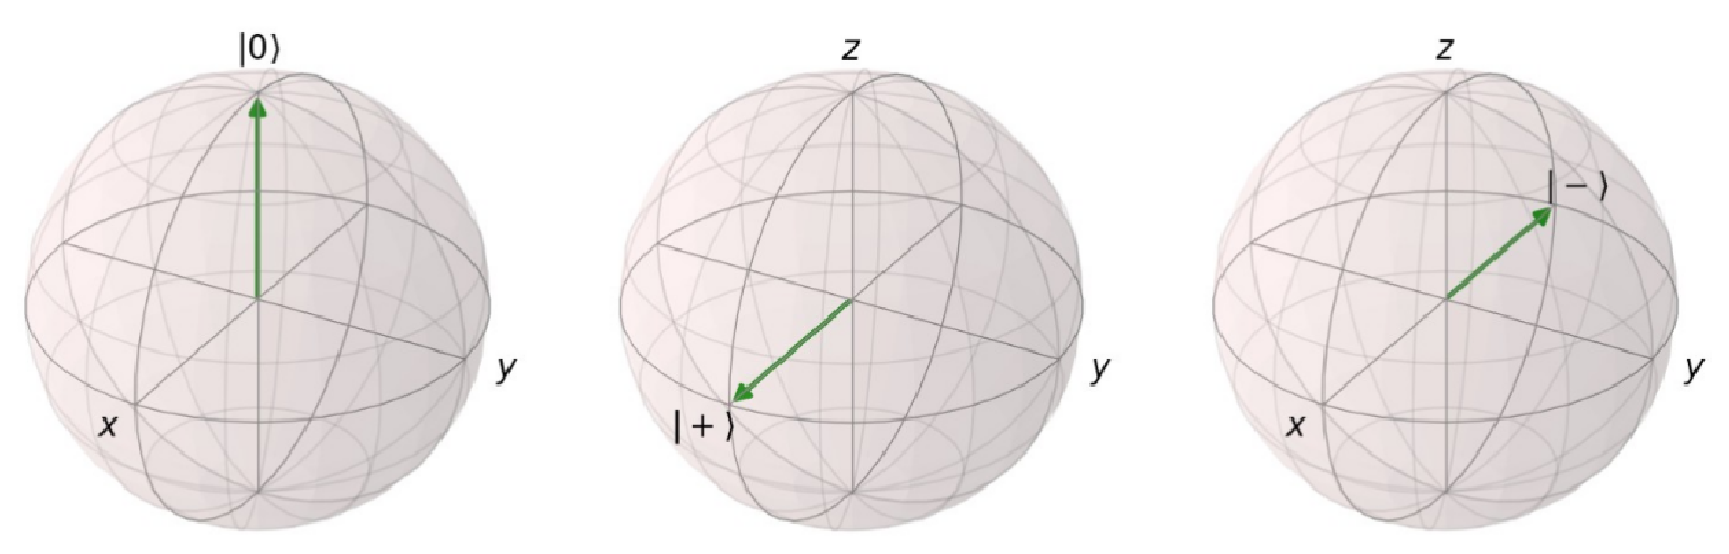
\includegraphics[scale=0.37]{images/simple_circuit.eps}
  \caption{States of our qubit throughout the circuit from left to right: \ket{0} $\rightarrow$ $H\ket{0}$ $\rightarrow$ $ZH\ket{0}.$}
  \label{fig:gate_rotations}
\end{figure}

\subsection{Vector Notation} \label{sec:matrix_notation}
Earlier we showed that we can represent a quantum state using the following formula:
\[\ket{\psi} = \alpha\ket{0} + \beta\ket{1}\]
The quantum states $\ket{\psi}$, $\ket{0}$ and $\ket{1}$ in the formula above are vectors. We define $\ket{0}$ and $\ket{1}$ as following:
\[\ket{0} = \qstatezero{}\]
\[\ket{1} = \qstateone{}\]
A quantum state has to be a normalized vector since we are talking probabilities, where $|\alpha|^2+|\beta|^2 = 1$. In general, a qubit's state is a unit vector in a two-dimensional complex vector space. A state can be written out as a linear combination:
\[
  \ket{\psi} = \alpha\qstatezero{} + \beta\qstateone{} =
\begin{bmatrix}\alpha \\ \beta\end{bmatrix}
\]
The single-qubit gates can then be represented by $2 \times 2$ unitary matrices:
\setlength\multicolsep{0pt}
\begin{multicols}{3}
  \[
    I = \igate{}
  \]
  \vfill
  \[
    X = \xgate{}
  \]
  \vfill
  \[
    Y = \ygate{}
  \]
\end{multicols}

\begin{multicols}{3}
  \[
    Z = \zgate{}
  \]
  \vfill
  \[
    H = \hgate{}
  \]
  \vfill
  \[
    S = \sgate{}
  \]
\end{multicols}
\bigskip
\noindent
Then a computation like $X\ket{0}$ can be calculated by matrix vector multiplication:
\[
X\ket{0} = \xgate{} \qstatezero{} = \qstateone{}
\]
And we find that $X\ket{0} = \ket{1}$. Or, more general:
\[
  X\begin{bmatrix}\alpha \\ \beta\end{bmatrix} = \begin{bmatrix}\beta \\ \alpha\end{bmatrix}
\]

You can combine quantum gates by multiplying their matrices. For example, let's verify that $H$ is self-inverse by applying it to itself:
\[
  H^2 = \hgate{} \hgate{} = \igate{} = I
\]
The result is the identity gate, showing that the inverse of $H$ is indeed itself. It is also a \emph{Hermitian matrix}, because it is equal to its own Hermitian adjoint: $H = H^\dagger$.

\newpage

\section{Fundementals: A Multi-Qubit World}
\subsection{The Step to Multi-Qubit}
We can represent multiple qubits using the \emph{Kronecker product}:
\[
  \ket{ab} = \ket{a} \otimes \ket{b} = \alpha_{00}\ket{00} + \alpha_{01}\ket{01} + \alpha_{10}\ket{10} + \alpha_{11}\ket{11}
\]
To represent \ket{00} for example:
\[
  \ket{00} = \ket{0} \otimes \ket{0} = \qstatezero{} \otimes \qstatezero{} =
  \begin{bmatrix}
  1\qstatezero{} \\[13pt]
  0\qstatezero{}
  \end{bmatrix}
  =
  \begin{bmatrix}
  1 \\
  0 \\
  0 \\
  0
  \end{bmatrix}
\]
Note that the size of the vector of two qubits is twice as big as the vector for one qubit. This is where some of the power of quantum computers comes from. With $n$ qubits you can represent $2^n$ states at the same time - an exponential growth from classical bits.

For multi-qubit states the rule remains that the state vector has to be normalized. For two qubits for example: $\alpha_{00}\ket{00} + \alpha_{01}\ket{01} + \alpha_{10}\ket{10} + \alpha_{11}\ket{11} = 1$. Or, more general, for a $n$ qubit state:
\[
\sum_{i}^{2^n} |\alpha_i|^2 = 1
\]

\subsection{Quantum State Evolution}
Doing single-qubit operations on a multi-qubit state is possible by combining the identity and our single-qubit gate. Say we want to compute $H_1\ket{0_0 0_1}$. That is, put the second qubit through a Hadamard gate.\footnote{Note that when I say ``second" qubit, I'm talking about the most right, or least significant qubit. I will number them for this example but assume it from here on out.} To do so, the gate matrix's column width has to be equal to the quantum state vector's dimension. We can achieve this by taking the Kronecker product of the identity matrix and our single-qubit matrix (in this case $H$):
\[
  H_1\ket{0_0 0_1} = (I_0 \otimes H_1)\ket{0_0 0_1}
\]
\newpage
\noindent
Writing it out:
\begin{align}
  I_0 \otimes H_1 &=
  \igate{} \otimes \hgate{} \\
  &=
  \dfrac{1}{\sqrt2}
  \left(
  \igate{}
  \otimes
  \begin{bmatrix}
  1 & \phantom{-}1 \\
  1 & -1
  \end{bmatrix}
  \right) \\
  &= \dfrac{1}{\sqrt2}
  \begin{bmatrix}
  1 & \phantom{-}1 & 0 & \phantom{-}0 \\
  1 & -1 & 0 & \phantom{-}0 \\
  0 & \phantom{-}0 & 1 & \phantom{-}1 \\
  0 & \phantom{-}0 & 1 & -1 \\
  \end{bmatrix}
\end{align}
Then we can put our \ket{00} state through it:
\[
  \dfrac{1}{\sqrt2}
  \begin{bmatrix}
  1 & \phantom{-}1 & 0 & \phantom{-}0 \\
  1 & -1 & 0 & \phantom{-}0 \\
  0 & \phantom{-}0 & 1 & \phantom{-}1 \\
  0 & \phantom{-}0 & 1 & -1 \\
  \end{bmatrix}
  \begin{bmatrix}
  1 \\
  0 \\
  0 \\
  0
  \end{bmatrix}
  =
  \dfrac{1}{\sqrt2}
  \begin{bmatrix}
  1 \\
  1 \\
  0 \\
  0
  \end{bmatrix}
\]
Which can also be written in Dirac notation as $\dfrac{1}{\sqrt2}(\ket{00} + \ket{01})$.

\subsection{Partial Measurement}
Say we want to measure the first qubit, $q_0$, in the following circuit:
\[
  \Large
  \Qcircuit @C=0.5em @R=0.5em @!R {
    \push{\rule{0em}{1.5em}} & & & & \lstick{q_0: \ket{0}} & \qw & \gate{H} & \qw & \meter & \cw \\
    \push{\rule{0em}{1.5em}} & & & & \lstick{q_1: \ket{0}} & \qw & \gate{H} & \qw & \qw & \qw \\
  }
\]
\noindent
First, we put both qubits in our state \ket{00} through a Hadamard gate. This puts it in the following state:
\[
  HH\ket{00} = \dfrac{1}{2}(\ket{00} + \ket{01} + \ket{10} + \ket{11})
\]
When we measure $q_0$ we have a 50/50 probability of getting a 0 or 1. We get either of the following states based on $M(q_0)$:
\[
  \ket{\psi} = 
  \begin{cases}
  \begin{aligned}
    \dfrac{1}{\sqrt2}(\ket{\uline{0}0} + \ket{\uline{0}1}) & \text{ if } M(q_0) = 0 \\
    \dfrac{1}{\sqrt2}(\ket{\uline{1}0} + \ket{\uline{1}1}) & \text{ if } M(q_0) = 1
  \end{aligned}
  \end{cases}
\]
We have two possible states after measurement, a state where $q_0$ is 0 or a state where $q_0$ is 1. Qubit $q_1$ will stay in superposition because we haven't measured that one. Notice how the first qubits (underlined) in both states are the same. This makes sense, we've measured that one so we're sure of its state.

\subsection{Common Two-Qubit Gates}
\subsubsection{CNOT Gate}
The quantum gate controlled-$NOT$ ($CNOT$, sometimes called $controlled-X$) is comparable to a classical computer's XOR, but it's reversible. This gate has two input qubits, the \emph{control} qubit and \emph{target} qubit. If the control qubit is set to 0, then the target qubit is left alone. If the control qubit is set to 1, then the target qubit is flipped. The circuit representation for $CNOT$ can be seen in Figure~\ref{fig:cnot_circuit}. Qubit $q_0$ represents the control qubit and $q_1$ represents the target qubit. It's essentially a Pauli $X$ gate with a control qubit. $CNOT$ is Hermitian and belongs to the Clifford gates.

\begin{figure}[ht]
\centering
\begin{minipage}{.45\textwidth}
  \[
    \Large
    \Qcircuit @C=0.5em @R=0.5em @!R {
	  \push{\rule{0em}{1em}} & & & &  \lstick{\ket{q_0}} & \ctrl{1} & \qw & \ctrl{1} & \qw \\
	  \push{\rule{0em}{1em}} & & & & \lstick{\ket{q_1}} & \targ & \qw & \gate{X} & \qw    \\
	}
  \]
  \caption{Circuit representations of $CNOT$. We will use the left representation.}
  \label{fig:cnot_circuit}
\end{minipage}%
\hspace*{.05\textwidth}
\begin{minipage}{.45\textwidth}
  \[
    U_{CN} = \cnotgate{}
  \]
  \caption{Matrix representation of $CNOT$.}
\end{minipage}
\end{figure}
\noindent
Let's look at an example of a $CNOT$ gate. Consider the following circuit:
\[
  \Large
  \Qcircuit @C=0.5em @R=0.5em @!R {
    \push{\rule{0em}{1.5em}} & & & & & \lstick{q_{0}: \ket{0}} & \gate{X}  & \ctrl{1} & \qw & \qw\\
    \push{\rule{0em}{1.5em}} & & & & & \lstick{q_{1}: \ket{0}} & \qw & \targ & \qw & \qw\\
  }
\]
First we put $q_0$ (the control qubit) in the \ket{1} state by applying an $X$ gate, giving us the state \ket{10}. Then we apply the $CNOT$ gate:
\[
  CNOT\ket{10} = \cnotgate{}
  \begin{bmatrix}
  0 \\
  0 \\
  1 \\
  0
  \end{bmatrix}
  =
  \begin{bmatrix}
  0 \\
  0 \\
  0 \\
  1
  \end{bmatrix}
  =
  \ket{11}
\]
The target qubit was flipped because the control qubit was set to 1, giving us \ket{11}.

\subsubsection{CZ Gate}
$CZ$, or the controlled-$Z$ gate, acts in a similar way to other controlled gates. That is, do the operation on the target qubit if the control qubit is set to 1, otherwise do nothing. In $CZ$ the operation is the Pauli $Z$ gate. $CZ$ is also Hermitian and belongs to the Clifford gates.
\begin{figure}[ht]
\[
  \Large
  \Qcircuit @C=0.5em @R=0.5em @!R {
    \push{\rule{0em}{1em}} & & \lstick{\ket{q_0}} & \ctrl{1} & \qw & \ctrl{1} & \qw \\
    \push{\rule{0em}{1em}} & & \lstick{\ket{q_1}} & \ctrl{-1} & \qw & \gate{Z} & \qw  \\
  }
\]
\caption{Circuit representations of $CZ$.}
\end{figure}

\subsubsection{Controlled Gates}
Controlled gates act on two or more qubits, where one or more qubits act as control for some operation. Generally, if $U$ is a gate that operates on single qubits with the following matrix representation:
\[
  U =
  \begin{bmatrix}
  u_{00} & u_{01} \\
  u_{10} & u_{11} \\
  \end{bmatrix}
\]
then the controlled-$U$ gate is a gate that operates on two qubits where the first qubit serves as control. The general matrix representation of the controlled-$U$ then looks as following:
\[
  C(U) =
  \begin{bmatrix}
  1 & 0 & 0 & 0 \\
  0 & 1 & 0 & 0 \\
  0 & 0 & u_{00} & u_{01} \\
  0 & 0 & u_{10} & u_{11} \\
  \end{bmatrix}
\]
\subsection{Toffoli Gate}
We can simulate a classical circuit using a quantum circuit. Most classical gates however are non-reversible. This is a problem for our quantum circuit, as it requires gates to be reversible. We can make use of a reversible gate known as the \emph{Toffoli gate} to make a quantum equivalent of any classical gate.

The Toffoli gate has three inputs and outputs (Figure \ref{fig:toffoli_circuit}), where two of the input qubits act as control bits. The third qubit is the target bit which is flipped if both control qubits are set to 1, otherwise it's left alone. For example, applying the Toffoli gate to the state \ket{110} flips the third qubit, resulting in the state \ket{111}.

\begin{figure}[ht]
\[
  \Large
  \Qcircuit @C=0.54em @R=1em @!R {
    \push{\rule{0em}{1em}} & & \lstick{a} & \ctrl{1} & \qw & a\\
    \push{\rule{0em}{1em}} & & \lstick{b} & \ctrl{1} & \qw & b\\
    \push{\rule{0em}{1em}} & & \lstick{c} & \targ & \qw & & & c \otimes ab\\
  }
\]
\caption{Circuit representation of the Toffoli gate, where $\otimes$ is addition modulo two.}
\label{fig:toffoli_circuit}
\end{figure}
\noindent
The Toffoli, or controlled-controlled-X ($CCX$) gate can be represented by a $8 \times 8$ matrix:
\[
  \begin{bmatrix}
  1 & 0 & 0 & 0 & 0 & 0 & 0 & 0\\
  0 & 1 & 0 & 0 & 0 & 0 & 0 & 0\\
  0 & 0 & 1 & 0 & 0 & 0 & 0 & 0\\
  0 & 0 & 0 & 1 & 0 & 0 & 0 & 0\\
  0 & 0 & 0 & 0 & 1 & 0 & 0 & 0\\
  0 & 0 & 0 & 0 & 0 & 1 & 0 & 0\\
  0 & 0 & 0 & 0 & 0 & 0 & 0 & 1\\
  0 & 0 & 0 & 0 & 0 & 0 & 1 & 0\\
  \end{bmatrix}
\]
It is a non-Clifford gate.
% Maybe: Show creating universal NAND gate with Toffoli gate

\subsection{Entanglement}
Two qubits are entangled if and only if the state of those two qubits can \emph{not be expressed as two individual states} (non-separable). Let's first take a look at a separable, or non-entangled state:
\[
  \ket{\psi} = \dfrac{1}{2}(\ket{00} + \ket{01} + \ket{10} + \ket{11})
\]
This state can be separated and expressed as the following two individual states:
\[
  \ket{\psi} = \dfrac{1}{\sqrt2}(\ket{0} + \ket{1}) \otimes \dfrac{1}{\sqrt2}(\ket{0} + \ket{1})
\]
However, consider the following state:
\[
  \ket{\psi} = \dfrac{1}{\sqrt2}(\ket{00} + \ket{11})
\]
This is an entangled state. It cannot be expressed as two individual states. How do we know if a state is entangled? We say two qubits are entangled if they have \emph{nonzero concurrence}. The concurrence of a state can be calculated using the following formula:
\[
  C(\ket{\psi}) = 2|\alpha_{00}\alpha_{11} - \alpha_{01}\alpha_{10}|
\]
We can check if our entangled state is indeed entangled:
\[
  C\left(\dfrac{1}{\sqrt2}(\ket{00} + \ket{11})\right) = 2\left|\dfrac{1}{\sqrt2}\left(\dfrac{1}{\sqrt2}\right)\right| = 1
\]
It has a non-zero concurrence, so we can say it's entangled. How about our non-entangled state?
\[
  C\left(\dfrac{1}{2}(\ket{00} + \ket{01} + \ket{10} + \ket{11})\right) = 2\left|\dfrac{1}{2}\left(\dfrac{1}{2}\right) - \dfrac{1}{2}\left(\dfrac{1}{2}\right)\right| = 0
\]
A concurrence of 0, so it is indeed not entangled.
\subsection{The Bell States}
The \emph{Bell states} are four maximally entangled quantum states of two qubits:
\[
\ket{\Phi^+} = \dfrac{1}{\sqrt2}(\ket{00} + \ket{11})
\]
\[
\ket{\Phi^-} = \dfrac{1}{\sqrt2}(\ket{00} - \ket{11})
\]
\[
\ket{\Psi^+} = \dfrac{1}{\sqrt2}(\ket{01} + \ket{10})
\]
\[
\ket{\Psi^-} = \dfrac{1}{\sqrt2}(\ket{01} - \ket{10})
\]
We can create a Bell state with the following circuit:
\[
  \Large
  \Qcircuit @C=0.5em @R=0.5em @!R {
    \push{\rule{0em}{1em}} & & & & & & \lstick{q_{0}: \ket{0}} & \qw & \qw & \gate{H} & \qw & \qw & \ctrl{1} & \qw  \\
    \push{\rule{0em}{1em}} & & & & & & \lstick{q_{1}: \ket{0}} & \qw & \qw & \qw & \qw & \qw &\targ & \qw \\
  }
\]
\begin{center}
\begin{tikzpicture}[thick]
\draw[black, -triangle 60] (0, 0.0) -- (-0.5, -0.7) node [below] {$\ket{\psi_0}$};
\draw[black, -triangle 60] (1.8, 0.0) -- (1.8, -0.7) node [below] {$\ket{\psi_1}$};
%\draw[black, -triangle 60] (3.8, 0.0) -- (3.8, -0.7) node [below] {$\ket{\psi_2}$};
\end{tikzpicture}
\end{center}
We start with our state \ket{00} at $\ket{\psi_0}$. We put $q_0$ through a Hadamard gate, giving us the state $\dfrac{1}{\sqrt2}(\ket{00} + \ket{10})$ at $\ket{\psi_1}$. Finally we $CNOT$ that state giving us the final Bell state $\dfrac{1}{\sqrt2}(\ket{00} + \ket{11})$.

The significance of Bell states becomes apparent when we start measuring qubits of a Bell state. Take the circuit we used before to create the Bell state $\dfrac{1}{\sqrt2}(\ket{00} + \ket{11})$ and measure both qubits.
\[
  \Large
  \Qcircuit @C=0.5em @R=0.5em @!R {
    \push{\rule{0em}{1em}} & & & & & & \lstick{q_{0}: \ket{0}} & \gate{H} & \qw & \ctrl{1} & \meter & \cw  \\
    \push{\rule{0em}{1em}} & & & & & & \lstick{q_{1}: \ket{0}} & \qw & \qw &\targ & \meter & \cw \\
  }
\]
You will find that the measurement results are correlated:
\[
M(q_1) = 0 \text{ if } M(q_0) = 0
\]
\[
M(q_1) = 1 \text{ if } M(q_0) = 1
\]
If you measure $q_0$ to be 0, $q_1$ will also be 0 and vice versa. Note that in our example entangled state they correlate as being equal, but for the entangled state $\dfrac{1}{\sqrt2}(\ket{01} + \ket{10})$ they correlate as being opposites (measuring $q_0$ as 0 means $q_1$ will be 1).
\end{document}
